\documentclass[11pt,english,twocolumn]{article}
\renewcommand{\familydefault}{\sfdefault}
\usepackage[T1]{fontenc}
\usepackage[utf8]{inputenc}
\usepackage{pslatex}
\usepackage[english]{babel}
\usepackage{blindtext}
\usepackage{setspace}
\usepackage{url}
\usepackage{amssymb}
\usepackage{complexity}
\usepackage[inline]{enumitem}

%Definitions from Simon's mya4.sty
% Set the paper size to A4
\setlength{\paperheight}{297mm}
\setlength{\paperwidth}{210mm}
% Define commands which allow the width and height of the text
% to be specified. Centre the text on the page.
\newcommand{\settextwidth}[1]{
\setlength{\textwidth}{#1}
\setlength{\oddsidemargin}{\paperwidth}
\addtolength{\oddsidemargin}{-\textwidth}
\setlength{\oddsidemargin}{0.5\oddsidemargin}
\addtolength{\oddsidemargin}{-1in}
}
\newcommand{\settextheight}[1]{
\setlength{\textheight}{#1}
\setlength{\headheight}{0mm}
\setlength{\headsep}{0mm}
\setlength{\topmargin}{\paperheight}
\addtolength{\topmargin}{-\textheight}
\setlength{\topmargin}{0.5\topmargin}
\addtolength{\topmargin}{-1in}
}
\addtolength{\topsep}{-3mm}% space between first item and preceding paragraph.
\addtolength{\partopsep}{-3mm}% extra space added to \topsep when environment starts a new paragraph.
\addtolength{\itemsep}{-5mm}% space between successive items.

%End of Simon's mya4.sty
\usepackage{graphicx}%This is necessary and it must go after mya4
\settextwidth{176mm}
\settextheight{257mm}
\usepackage[usenames,dvipsnames,svgnames,table]{xcolor}
\def\baselinestretch{0.95}

\usepackage[compact]{titlesec}
\titlespacing{\section}{0pt}{*1}{*1}
\titlespacing{\subsection}{0pt}{*1}{*0}
\titlespacing{\subsubsection}{0pt}{*0}{*0}
\titlespacing{\paragraph}{0pt}{*0}{*1}
\titleformat*{\paragraph}{\itshape}{}{}{}
%% --------------------------------------------------------------------------------------------------------------------------------
\begin{document}
\title{Abstraction in First-Order Probabilistic Inference}

\author{Paulius Dilkas (2146879)}
\date{}
\maketitle

\section{Proposed Research}

\subsection*{Background} % half of page

%\begin{figure*}
%  \centering
%  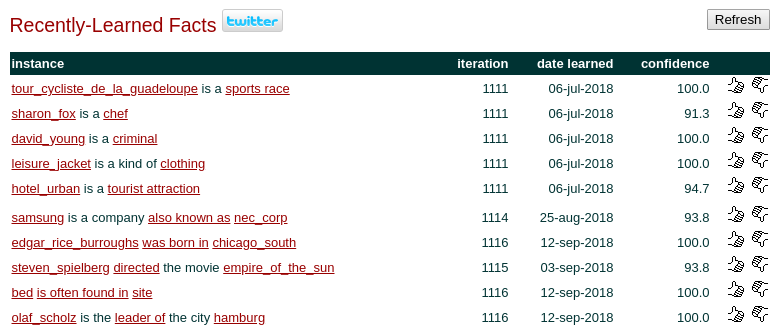
\includegraphics[width=\textwidth]{nell.png}
%  \label{fig:nell}
%  \caption{Relational facts learned from browsing websites by a continuous
%    language learning system NELL
%    \cite{DBLP:conf/aaai/CarlsonBKSHM10,DBLP:journals/cacm/MitchellCHTYBCM18}
%    (screenshot from the project's
%    website \protect\url{http://rtw.ml.cmu.edu/rtw/}).}
%\end{figure*}

% uses: formal methods for model checking
% curry-howard isomorphism/correspondence => applications in programming
% language types, semantic web
%Furthermore, the
%Curry-Howard isomorphism shows how type inference in a programming language can
%be equivalent to proofs in logic \cite{DBLP:journals/cacm/Wadler15}.
% automated theorem proving, proof checking, interactive theorem proving

Logical approaches to reasoning have dominated the fields of artificial
intelligence (AI) and computing for many decades. They have resulted in expert
systems that can use reasoning to make predictions and diagnose problems
\cite{hayes1983building}, logic programming languages that allow the user to
declaratively describe the problem and trust the inference algorithm to find the
answer efficiently \cite{DBLP:books/sp/Lloyd87}, and automated (interactive)
theorem proving and proof checking software that assists mathematicians in
constructing correct proofs \cite{DBLP:books/el/RobinsonV01}. Probabilistic
methods, on the other hand, have particularly flourished with the arrival of big
data and access to more data in general, transforming areas such as natural
language processing and pattern recognition \cite{DBLP:series/sci/BrazAR08}.

While probabilistic models are great at handling uncertainty, their
simplistic representations can be hard to interpret. On the other hand, systems
based on logic have rich representations, but cannot handle uncertainty.
\emph{First-order probabilistic inference} (FOPI) (also known as
\emph{statistical relational AI}) attempts to bridge the gap
between the two and suggests a range of representations\footnote{ We will
  sometimes refer to FOPI models as \emph{probabilistic relational models},
  since relations play an important part in this richer representational
  structure.} capable of handling probabilities as well as (parts of)
first-order logic \cite{DBLP:series/sci/BrazAR08}. The models can be constructed
manually or learned from data, and the process of computing the probability of a
query---usually in the form of a random variable, possibly conditioned on other
random variables---is called \emph{inference}.

Most of these models are based either on adding probabilities to programming
languages or on adding richer representational structure to probabilistic
graphical models (PGMs). The former kind is called \emph{probabilistic
  programming} \cite{DBLP:conf/icse/GordonHNR14} and is an active area of
research with many implementations. A well-known example is \emph{ProbLog}
\cite{DBLP:conf/ijcai/RaedtKT07}---a language that extends the logic programming
language Prolog by attaching a probability to every clause in the program. A
prominent example of the latter is a \emph{Markov logic network} (MLN)
\cite{DBLP:journals/ml/RichardsonD06}, which is simply a collection of
first-order statements (formulas), with a weight attached to each statement.
MLNs were proposed as a first-order generalisation of \emph{Markov random
  fields}---an undirected PGM. We will use MLNs to provide concrete examples,
but we do not commit ourselves to a specific FOPI model just yet.

As an area of research, FOPI is a subfield of AI and can be thought as the
probabilistic cousin of automated reasoning. The problem of learning a FOPI
model from data draws the attention of researchers not only from the machine
learning community, but also data mining and knowledge discovery. Due to how
many of the models are formulated, there is also significant overlap with
research in programming languages and, specifically, logic programming.

In the last decade, we have seen applications of FOPI in a wide range of areas,
ranging from toy problems in probability one might find in a textbook
\cite{DBLP:conf/ijcai/DriesKDBR17} all the way to genetics
\cite{DBLP:journals/jcb/SakhanenkoG12} and cancer research
\cite{DBLP:conf/ilp/Corte-RealD017}. For instance, probabilistic relational
structures have been integrated into recommendation systems
\cite{DBLP:journals/corr/YangKAGN16} and stream mining software
\cite{DBLP:conf/icdm/ChandraSKTA14}, and various FOPI models have been used to
predict the remaining lifetime of hardware components
\cite{vlasselaer2012statistical} as well as patterns of criminal and terrorist
activity \cite{DBLP:conf/sdm/DelaneyFCWJ10}. Moreover, one type of probabilistic
logic has been extended to explicitly deal with changes over time and has been
used to model virtual spaces such as online chat rooms and massively multiplayer
online games \cite{DBLP:conf/pkdd/ThonLR08,DBLP:journals/ml/ThonLR11}.

\subsection*{Key Idea} % half of page

\emph{``To investigate how first-order probabilistic models can be transformed
  into more abstract representations without losing (significant) detail
  crucial to the set of relevant queries.''}

\emph{Abstraction} can be broadly defined as the process (and result) of
omitting detail \cite{doi:10.1086/670300}. Sometimes the omitted information is
irrelevant in answering the questions we are interested in, and sometimes an
abstraction provides a simplified (and approximately correct) view of a
situation that originally was too complex to be reasoned about. While areas such
as planning and verification have benefited from abstraction in various ways
\cite{saitta2013abstraction}, research into abstraction in FOPI has just begun
and awaits significant contributions
\cite{DBLP:journals/corr/abs-1810-02434,DBLP:conf/icml/HoltzenBM18,DBLP:conf/uai/HoltzenMB17}.

Our goal is to develop new types of abstractions, find efficient
algorithms for constructing an abstraction from a given model, and investigate
how abstraction can be integrated into both inference and learning algorithms.
Simplification and abstraction can benefit us in both efficiency and
interpretability, i.e, simpler models are likely to result in faster inference,
while at the same time being easier to understand by the user. Finally, the
quest for abstraction algorithms is likely to lead to a better theoretical
understanding of what properties can be preserved by an abstraction, what error
bounds can be established when abstraction approximates the answer, and upper
and lower bounds on the complexity of performing abstraction and providing the
desired guarantees.

%This is an interesting line of research because seeking simplicity is in line
%with philosophical principles such as Occam's razor. It is also important
%because of the likely improvements in inference speed. In a way, a significant
%line of research for faster inference focusing on \emph{lifted inference} can be
%seen as a special case of abstraction.

%TODO: main benefit

\subsection*{Objectives}

\begin{itemize}
\item To further the theoretical understanding of abstraction in FOPI.
\item To improve inference speed by investigating abstraction as a separate
  process as well as a component of inference.
\item To make models learned from data simpler and more transferable.
\item To increase the explainability of FOPI models.
\end{itemize}

\subsection*{State of the Art} % one page

\subsubsection*{Inference}

Recall that a ProbLog program is a set of clauses, where each clause has an
associated probability. The ProbLog inference rule
\cite{DBLP:series/synthesis/2016Raedt,DBLP:conf/iclp/Sato95} for calculating the
probability of an arbitrary query $Q$ being true is
\[
  P(Q) = \sum_{F \models Q} \prod_{f \in F} P(f) \prod_{f \not\in F} 1 -
  P(f).
\]
Here, we are summing over all instantiations of variables (called \emph{possible
worlds}) that satisfy the query, where $F$ denotes a set of clauses that are
evaluated as true. For each world, we calculate its probability by multiplying
probabilities associated with clauses or their negations. With this
definition, the inference problem becomes an instance of weighted model
counting \cite{DBLP:series/synthesis/2016Raedt}.

\emph{Weighted model counting} (WMC) is an extension of model counting, which is
an extension of the \emph{Boolean satisfiability problem} (SAT)
\cite{DBLP:journals/ai/ChaviraD08}. SAT asks whether one can assign values to
variables so that a given formula evaluates to true. Model counting asks to
count the number of ways that can be done. Weighted model counting further
extends this problem by assigning a weight to each possible world (in whatever
way is appropriate for the problem) and asks for the sum of the weights
corresponding to all possible worlds where the formula (or query) is true. In
the case of ProbLog, the weight of a world is the product of probabilities of
all literals (whether evaluated/instantiated to true or false)
\cite{DBLP:series/synthesis/2016Raedt}. The WMC instance is then compiled to
some type of logical circuit for efficient inference. \emph{Knowledge
  compilation} \cite{DBLP:conf/ijcai/BroeckTMDR11} is the state-of-the-art
inference technique for PGMs as well as many FOPI models
\cite{DBLP:series/synthesis/2016Raedt}.

Inference for MLNs works in a similar way. We still sum over all possible
worlds where the query is true, but the probability of a world $x$ is now
defined as
\[
  P(x) = \frac{1}{Z} \exp \left( \sum_{i=1}^F w_i n_i(x) \right),
\]
where $Z$ is the normalising constant more commonly known as the \emph{partition
function}, $F$ is the number of formulas in the MLN, $w_i$ is the weight of the
$i$th formula, and $n_i(x)$ is the number of ways that formula $i$ can be
grounded in order to satisfy world $x$. Here, \emph{grounding} a formula refers
to replacing each variable with a value so that the formula evaluates to true.

A commonly used inference algorithm for MLNs relies on \emph{probabilistic
  theorem proving}
\cite{DBLP:journals/cacm/GogateD16,DBLP:journals/cib/Venugopal17}
which is an example of a \emph{lifted inference} algorithm, i.e., an algorithm
that attempts to work directly with variables without having to consider every
possible value \cite{DBLP:conf/ijcai/Poole03}. The underlying problem, however,
is still WMC, and is solved using a combination of techniques well established
in the SAT community, e.g., unit propagation and clause learning
\cite{DBLP:journals/cib/Venugopal17}.

%Lifting is performed in two ways: lifted decomposition (identifying identical
%and independent FO components). Lifted conditioning. Without lifting, computing
%a conditional probability that depends on a predicate would require computing a
%probability for each \emph{grounding} of that predicate. Instead, we can
%partition groundings into equivalence classes, where all groundings in an
%equivalence class behave in exactly the same way and thus produce the same
%answer.
%Another interesting development is led by a team at SRI International that
%considers probabilistic inference in a generalised (modulo theories) manner
%\cite{DBLP:conf/ijcai/BrazOGD16}, including a recent improvement
%\cite{DBLP:conf/uai/BrazO17} that makes the algorithm support relations and
%widens the range of situations where the algorithm acts in a lifted manner.

\subsubsection*{Abstraction}

Abstraction is an important tool in human cognition and a well-studied subject
in cognitive science. For example, Gentner and Hoyos \cite{Gentner2017-GENAAA-2}
investigate how children learn abstract patterns from observing several
objects with a common property, while Bransford and Franks
\cite{BRANSFORD1971331} show how the idea conveyed by a sentence is abstracted
away from the particulars of its syntactic expression.

Abstraction is also well-known in the AI community,
where the main goal of abstraction is to reduce the computational complexity of
a task, while ensuring that the process of abstraction itself is reasonably
efficient \cite{saitta2013abstraction}. For instance, abstraction plays a key
part in modern approaches to planning, where compound tasks are used to abstract
away the details of how those tasks can be implemented
\cite{DBLP:journals/amai/ErolHN96}. More specifically, abstraction is essential
in developing explainable AI \cite{DBLP:journals/access/AdadiB18}, where
it has been used to create interpretable abstractions of observed behaviour
\cite{DBLP:journals/corr/PenkovR17} and model the domain knowledge of the user
as an abstraction of the system, thus producing explanations that are at the
level of detail corresponding to the user's knowledge
\cite{DBLP:conf/ijcai/SreedharanSK18}.

Model checking and verification benefit from abstraction as well, particularly
in the area of software verification, where a complete model of the program
might be too big to be handled by even the most efficient methods, in which
case an abstract model could be developed. Depending on how it is created,
sometimes properties of the system can be verified using the abstraction
\cite{DBLP:journals/toplas/ClarkeGL94}, while other times the abstract model
might produce a false positive, i.e., signal about a possible problem where
there is none. If the occurrence of a false positive is suspected, parts of the
abstraction can be refined to provide the necessary level of detail, while
keeping other parts as they were
\cite{DBLP:conf/cav/ClarkeGJLV00,DBLP:conf/popl/HenzingerJMS02}.

Probabilistic abstractions have been used in the context of software
verification, where probabilities can help the verification algorithm choose
which part of the abstract model needs to be refined
\cite{DBLP:conf/pldi/ZhangSN17}. Meanwhile, in the probabilistic programming
community, abstractions have been used to determine the required number of Monte
Carlo samples in order to compute a probability within a required level of
precision \cite{DBLP:conf/popl/Monniaux01}.

However, only recently has the general case of abstraction for FOPI models been
formalised, and the work is mostly limited to defining several key properties
that an abstraction may have and showing how those properties interact with each
other \cite{DBLP:journals/corr/abs-1810-02434}. While the work on probabilistic
programming considers specific examples of abstractions
\cite{DBLP:conf/uai/HoltzenMB17} and presents an algorithm for performing
predicate abstraction \cite{DBLP:conf/icml/HoltzenBM18}, significant work is
required to achieve the full generality outlined in this proposal.

\subsection*{Our Solution} \label{section:our_solution} % 0.5-1 page

While some theoretical groundwork for abstraction in FOPI has recently been
developed by Belle \cite{DBLP:journals/corr/abs-1810-02434}, there are many
questions left to be answered:
\begin{enumerate}
\item How to efficiently create an abstraction of an already-existing
  model? \label{q:1}
\item When is the correct time to stop? What is the right balance between
  simplicity and information? \label{q:2}
\item What makes one abstraction preferable to another? \label{q:3}
\item How to incorporate abstraction steps into learning a model from
  data? \label{q:4}
\item How to provide guarantees about an abstraction? For example, we may want
  to bound the error of an answer to any query, or to ensure that all answers
  remain exact for a selected set of queries. \label{q:5}
\end{enumerate}

In order to answer these questions and develop the required algorithms and
techniques, we can draw inspiration from the theory of abstraction for reasoning
in formal systems developed by Giunchiglia and Walsh
\cite{DBLP:journals/ai/GiunchigliaW92} and recent work on abstraction for
structural equation models \cite{DBLP:conf/uai/RubensteinWBMJG17}. In
particular, an abstraction is often defined as a transformation of the
representation into a different form. One way to create such a transformation is
via a composition of atomic operations. For example:
\begin{itemize}
\item In some cases, $a \rightarrow b$ and $b \rightarrow c$ can be simplified
  to $a \rightarrow c$.
\item If a statement $S$ is true with high probability, perhaps that probability
  can be rounded up to $1$, eliminating the need to consider the case where $S$
  is false.
\item If a statement is true for all values of a variable, barring a few
  exceptions, perhaps the exceptions can be discarded.
\end{itemize}

Consider a specific query $Q$. Applying such an abstraction rule may or may not
change the answer to $Q$, depending on whether the removed information
is relevant to the query. Even if the answer becomes less precise, it might be
an acceptable approximation, given that the error is bounded to a reasonable
degree. Either way, the abstraction can reduce the search space the inference
algorithm has to explore in order to produce an answer.

It becomes clear that it is important to consider creating abstractions with
respect to a specific set of queries. Question \ref{q:5} can then be answered by
considering how each abstraction rule affects different types of queries.
Sometimes we may get a reasonable numerical upper bound on the error, while
other times it may be too time-consuming (or impossible) to bound the error to
any reasonable degree, forcing us to reject the abstraction rule altogether.

Thus, we will develop a comprehensive list of abstraction rules
(transformations) and define a way to categorise all queries answerable by a
FOPI model such that we could answer the following set of questions for each
abstraction rule:
\begin{itemize*}
\item What types of queries can no longer be answered exactly after applying the
  abstraction rule?
\item What is the error bound? Can it be calculated in constant time?
\item What is the complexity of applying the abstraction?
\end{itemize*}

Questions \ref{q:2} and \ref{q:3} delve deeper into how an abstraction algorithm
could work. If the set of rules is extensive enough, any model might
eventually be oversimplified into something trivial. We need to measure two
things: the amount of (relevant) information preserved by an abstraction, and
the complexity of the model. The two metrics would provide a systematic way to
answer both questions, while being easily adaptable to different needs (e.g.,
how much precision are we willing to sacrifice? What queries do we want to
support?).

Lastly, we will integrate abstraction steps into both inference and learning
algorithms, resulting in faster inference as well as simpler and more robust
models.

\subsection*{Innovative Aspects} % 0.25 page

We aim to innovate by expanding the idea of abstraction in AI to new domains as
well as enhancing both inference and learning of probabilistic relational
models.

\paragraph{Abstraction in AI} The work on abstraction so far has focused almost
exclusively on deterministic systems. We will extend previous work to target
rich probabilistic models, resulting in new theoretical ideas and definitions as
well as algorithms for transforming models into their abstractions.

\paragraph{FOPI} As FOPI subsumes both probabilistic inference (often
$\#\P$-complete) and logical inference (\NP-complete)
\cite{DBLP:journals/ml/RichardsonD06}, it is unlikely that a useful variation of
FOPI can ever be tractable. Thus, improvements in inference speed are highly
desirable. We will integrate abstraction steps into inference algorithms,
making the algorithm recognise opportunities to reduce the complexity of the
model before continuing the search. This is likely to yield significant benefits
to inference speed.

\paragraph{Statistical relational learning} Abstraction can also be integrated
into learning a FOPI model from data. This is likely to make the model more
understandable to the user as well as increase the transferability of the model
to previously unseen data.

\section{Methodology} % 1.5 pages

\subsection*{Comparative Survey of FOPI Models (WP1)}

As there is no consensus over the quality and capabilities of various
FOPI models, we will develop a list of problems that can be used to compare and
challenge state-of-the-art inference algorithms for various representations. We
will draw inspiration from problems that already exist in the literature and
have been used to propose new approaches, e.g., the classic `a friend of a
smoker is likely to be a smoker' example commonly used to introduce FOPI
representations
\cite{DBLP:series/sci/BrazAR08,DBLP:conf/ijcai/BroeckTMDR11,DBLP:journals/ml/RichardsonD06,DBLP:journals/cib/Venugopal17}
and the urn-and-balls scenario that requires handling uncertainty about the
number of objects and their identities \cite{DBLP:conf/ijcai/MilchMRSOK05}.
These and other example problems will allow us to compare modern FOPI models
in terms of what complexities of the problem can be represented in a reasonable
way, and efficiency of inference (both empirical and in terms of computational
complexity). \textbf{Deliverable:} a report with a list of problems, indication of
which representations are able to solve each problem, the computational
complexity of each solution, and plots comparing the performance of different
models for each problem.

\subsection*{Abstraction Rules and Their Properties (WP2)}

Developing a list of abstraction rules (transformations) that can be composed to
achieve any (even a trivial) abstraction is an important step in our proposal.
While some examples have already been mentioned here and more can be found in
previous work
\cite{DBLP:journals/corr/abs-1810-02434,DBLP:journals/ai/GiunchigliaW92,DBLP:conf/uai/HoltzenMB17,saitta2013abstraction},
our aim is to develop a complete list of abstraction rules that are able to
simplify individual snippets of first-order logic, their probabilities, and
interactions among two or more snippets. After constructing such a list, we will
investigate whether (or to what extent) it satisfies several key properties (the
first three as defined by Belle \cite{DBLP:journals/corr/abs-1810-02434}):

\begin{description}
\item[Soundness] Do events that were possible before the abstraction stay
  possible?
\item[Completeness] Were events that are possible after applying the abstraction
  possible before?
\item[Exactness] Are all computable probabilities in the abstraction equal to
  the corresponding probabilities before the abstraction was applied?
\item[Commutativity] Can the order of two transformations be changed without
  changing the result?
\item[Thoroughness] Is the list of abstraction rules extensive enough to
  simplify any model into a trivial one? It is unlikely that we would do so in
  practice, but the list should be rich enough to support that.
\end{description}

\textbf{Deliverables:} a report detailing a list of abstraction rules, their
properties, and the required proofs as described above.

\subsection*{Applying Abstraction Rules in Practice (WP3)}

We will build on the work produced in the previous WP to bring the theory closer
to a useful implementation. Specifically, we will decide on a particular
internal representation for our chosen FOPI model in order to achieve efficient
application of abstraction rules. We will implement algorithms for applying each
rule, consider their computational complexity, and detail our findings in a
report with pseudocode snippets and investigations into the efficiency of
applying each transformation. \textbf{Deliverables:} a working implementation
featuring internal data structures, some example problems, and algorithms for
applying abstraction rules; a report describing our findings.

\subsection*{Ensuring a Sufficient Level of Precision (WP4)}

While knowing which abstraction rules are exact is useful, we would also
like to ensure that non-exact rules maintain a sufficient level of precision.
For each such rule, we will describe what queries can no longer be answered
exactly after applying the rule. Then, we will construct algorithms to bound the
error caused by the rule, and investigate their performance in terms of
computational complexity as well as empirical studies. \textbf{Deliverables:} a
report detailing how non-exactness affects classes of queries, implementation of
error-bounding algorithms, their theoretical and empirical analysis.

\subsection*{Greedy Algorithms (WP5)}

At this point, we can reason about applying multiple abstraction rules in
sequence. We will aim to answer two key questions:
\begin{itemize*}
\item How to choose which abstraction rule should be applied first?
\item When is the correct time to stop simplifying things?
\end{itemize*}
Exploring different answers to these questions will result in a set of
abstraction algorithms. As we expect most abstraction rules to commute with one
another, making the order the rules are applied in immaterial, we will focus on
\emph{greedy} algorithms, where we choose which abstraction rule should be
applied on a model based solely on the current state of the model.

Each algorithm will take a model, a description of a set of queries that need to
be supported, and an indication of how much loss in precision (if any) the user
is willing to tolerate. We will explore a variety of heuristics that establish
preferences over which abstraction rule should be applied first as well as
termination conditions. For instance, we could always pick an abstraction rule
that results in a model with highest entropy (similar ideas have been very
successful in reinforcement learning \cite{DBLP:conf/aaai/ZiebartMBD08}), or
prefer rules that have little effect on precision. While a natural termination
condition could be an inability to apply an abstraction rule without losing too
much precision, the process could also be terminated because either the loss in
precision or the expected running time of applying the abstraction is too high
for the predicted benefits in inference speed. \textbf{Deliverables:}
implementations of the algorithms as well as one or more papers detailing the
reasoning behind design decisions, observed empirical performance, and the
differences in inference speed before and after running each algorithm.

\subsection*{Abstraction During Inference (WP6)}

There is no reason to limit abstraction to the intermediate stage between
constructing (or learning) a model and performing inference. Thus, we will
investigate how the state-of-the-art inference algorithm for our chosen FOPI
model can benefit from performing abstraction steps throughout its execution.
For example, a common way to compute a conditional probability $P(Q \mid E)$
inside a model $\Delta$ using WMC is by calculating the WMC of $\Delta \land Q
\land E$ and $\Delta \land E$ separately, and then dividing one by the other
\cite{DBLP:journals/ai/ChaviraD08}. It is likely that the two computations would
benefit from different abstractions. \textbf{Deliverables:} an implementation of a
new inference algorithm with abstraction, and a report describing its design and
performance.

\subsection*{Abstraction in Learning (WP7)}

A learned model is, in a way, an abstraction of the training data. Performing
abstraction afterwards is suboptimal, since the algorithm would attempt to
stay close to the learned model rather than the underlying data itself. While
learning algorithms already measure goodness of fit, the measure will have to be
combined with a meaningful measure of simplicity in order to provide a
reasonable balance between the two. The abstraction rules themselves will need
to be rethought in the context of data, as abstraction ought not to be added at
the end as an extra step, but rather a fully integrated part of the learning
process that concerns itself primarily with a meaningful and accurate
representation of data. The abstraction ideas developed in previous work
packages will help ensure that the learned models are both more explainable and
transferable to new kinds of data. \textbf{Deliverables:} an implementation of a
learning algorithm with integrated abstraction, and a report describing the
rationale for its design as well as observed performance.

\subsection*{Dissemination (WP8)}

We will make the implementations of abstraction, inference, and learning
algorithms (as well as the newly constructed test data) publicly available in a
repository. A website dedicated to the project will provide a coherent view of
all developments as they are being implemented and written. We will aim to
produce a series of papers detailing both theoretical contributions and
empirical results in journals and conferences such as JAIR, UAI, IJCAI, AAAI,
NeurIPS, etc. \textbf{Deliverables:} project website, code repository,
dissemination activities.

\section{Measurable Outcomes}

\begin{itemize}
\item A set of problems delineating the differences amongst various
  representations as well as guiding future research efforts (WP1).
\item Demonstrated increase in exact and approximate inference speed (WP6).
\item Demonstrated improvement in models learned from data in terms of
  simplicity and transferability without (significant) loss in precision (WP7).
\end{itemize}

\section{Risks} % 0.25 page

Creating a new algorithm always carries a risk that the algorithm may not
perform well compared to what has already been achieved. Fortunately, previous
work, which features a very limited version of abstraction, shows promising
results in terms of reduction in inference speed
\cite{DBLP:conf/icml/HoltzenBM18}. We are confident that we can observe
similarly successful results with a much broader range of abstractions. In any
case, the project will result in valuable theoretical contributions regardless
of how well the ideas perform in practice.

Another risk is related to integrating abstraction into inference. Namely, it
might take too much time to create the abstraction compared to the time saved
during inference. Even if this turns out to be the case, the developed
abstraction algorithms would still be useful for models that are constructed
once and used to perform many inferences. However, the observed reductions in
inference speed seem to reduce the complexity of the task
\cite{DBLP:conf/icml/HoltzenBM18}, while at least some abstraction rules can
definitely be implemented in linear time. This suggests that with a big enough
model the gains in inference speed should eventually overtake the time taken to
construct the abstraction.

\section{Impact and National Importance} % 0.5 page

\paragraph{National Importance}

Our proposal covers an EPSRC growth area for statistics and applied probability
as well as several maintenance areas such as AI technologies, logic and
combinatorics, and theoretical computer science. Furthermore, our work will
contribute to areas such as big data (as more scalable inference will allow
expressive probabilistic models to be used with more data) as well as other
scientific disciplines (as both abstraction and richness of representation are
important topics in social sciences and medicine). Moreover, abstraction for
FOPI models is a new yet promising research area
\cite{DBLP:conf/icml/HoltzenBM18} which is likely to see many major
developments.

\paragraph{Impact}

The survey will highlight the weaknesses of current approaches and direct future
research towards open problems. Furthermore, many of the basic ideas behind
abstraction for a particular model are likely to be transferable to many others,
perhaps even inspiring a unifying theory behind all representations. Moreover,
making the models more efficient and explainable should also make them more
attractive to a larger user base, both academic and industrial.

\let\oldbibliography\thebibliography
\renewcommand{\thebibliography}[1]{\oldbibliography{#1}
\setlength{\itemsep}{-3pt}}

\bibliographystyle{abbrv}
%\setstretch{0.8}
{
\scriptsize
\bibliography{proposal}
}
\end{document}
